\documentclass{article}
\input{../../../../../LaTex/preamble/preamble_article.tex}


\title{热学总复习}
\author{学生: 杨凤 $\quad$ 教师: 马祥芸}


\begin{document}
\maketitle
\tableofcontents
\zihao{-4}
\newpage

\section{热力学}
\subsection{分子动理论}
\subsubsection{物体是由大量分子构成的}
\begin{enumerate}
    \item 分子的大小
          \begin{enumerate}[label = (\arabic*{})]
              \item 分子直径数量级: $10^{-10} \, m$
              \item 分子质量数量级: $10^{-26} \, kg$
              \item 测量分子的方法: 油膜法
          \end{enumerate}

          \vspace{2em}

    \item 两种分子模型
          \begin{enumerate}[label = (\arabic*{})]
              \item 球体模型: 认为分子是一个个紧挨着的球体(适用对象: 固体,液体;体积:$V = \frac{4\pi}{3} R^{3}$)
              \item 立方体模型: 认为分子是一个个紧挨着的立方体(适用对象: 气体;体积:$V = d^{3}$)
          \end{enumerate}

          \vspace{-1em}
          \hspace{1em}\begin{adjustbox}{minipage=0.86\linewidth, bgcolor=gray!20, padding=1em}
              \small
              固液相使用球体模型更为准确,气相使用立方体模型更为准确,这里的立方体空间是气体分子的活动空间
          \end{adjustbox}
          \vspace{-1em}

          \vspace{2em}

    \item 油墨法测量分子的直径
          \begin{itemize}
              \item 思路: 第一滴油酸摊开在水面上,近似看成单分子层
              \item 模型: 认为油酸分子为球体模型
              \item 要点:
                    \begin{itemize}
                        \item $1ml$油酸溶液配制成$500ml$油酸酒精溶液
                        \item 取$100$滴油酸酒精溶液测得体积为$1ml$
                        \item 先对水撒痱子粉,后滴液解决油膜的透明问题
                        \item 往水面上注射一滴油酸酒精溶液
                        \item 稳定后使用玻璃板盖进行描边
                        \item 使用\textbf{格子法}来计算不规则面积(不足半格取$0$,超过半格取$1$)
                    \end{itemize}
          \end{itemize}

          \vspace{2em}

          \subsubsection{微观量的估算}
          \begin{enumerate}[label = (\arabic*{})]
              \item 分子层面: 单个分子质量$m_{0}$,单个分子所占空间体积$V_{0}$
              \item 化学层面: 摩尔质量$M_{mol} \, (g \slash mol)$,摩尔体积$V_{mol} \, (L \slash mol)$
              \item 实际层面: 质量$M$,体积$V$
              \item[] 物理量之间的关系: $n = \frac{N}{N_{A}} \, mol \, (N_{A} = 6.02 \cross 10^{23})$
                  $$
                      M_{mol} = \frac{M}{n}   \quad   m_{0} N_{A} = M_{mol}
                  $$
                  $$
                      V_{mol} = \frac{V}{n}   \quad   V_{0} N_{A} = V_{mol} \quad
                  $$
                  $$
                      \hspace{0.2em} \text{摩尔体积适用于固液相,但是计算出来的并不能视作单分子体积,而是单分子占用空间}
                  $$
                  $$
                      \text{摩尔体积不适用于气体,因为标况下气体为}22.4L\text{,那么除以}N_{A}\text{会导致每个分子一样大}
                  $$

                  \vspace{-1em}
                  \hspace{-1em}
                  \begin{adjustbox}{minipage=0.38\linewidth, bgcolor=gray!20, padding=1em}
                      \small % 将字号变小为 small
                      标况: $0^{\circ}C$,一个标准大气压(约$101kPa$)
                  \end{adjustbox}

              \item[] 密度: 区分 \, 分子密度 \, 与 \, 气体密度,利用气体密度所求体积为 \,分子所占空间体积
          \end{enumerate}

\end{enumerate}

\vspace{2em}

\subsubsection{扩散现象和布朗运动}
一切物质的分子都在不停地做无规则的(热)运动

\begin{enumerate}
    \item 扩散现象
          \begin{enumerate}[label = (\arabic*)]
              \item 定义: 相互接触的不同物质能够彼此进入对方

                    \hspace{2.7em}此现象并不是宏观受力的作用下发生的,且各个状态下都会存在扩散现象
              \item 前提: 浓度差(梯度)
              \item \textbf{直接}反映了分子的无规则运动
              \item 扩散现象的快慢: 与物质的状态与温度有关,气体$>$液体$>$固体
          \end{enumerate}
    \item 布朗运动
          \begin{enumerate}[label = (\arabic*)]
              \item 定义: 悬浮在液体或(气体)中的微粒(宏观层面)的无规则运动
              \item 实验背景: 布朗看水中的花粉(显微镜)
              \item 观察结论: 微粒越小或温度越高,布朗运动越强烈
              \item 原因: 水分子对布朗微粒撞击的不平衡(不均匀)
              \item 布朗运动\textbf{不是}分子运动,\textbf{间接}反映了分子的无规则运动
          \end{enumerate}
    \item 扩散与布朗运动的混淆点
          \begin{enumerate}[label = (\arabic*)]
              \item 扩散现象: 微观力作用,宏观现象肉眼可见
              \item 布朗运动: 宏观力作用,宏观现象光学显微镜观察可见($10^{-6}$)
              \item 两者都是微观层面的分子无规则运动所形成的宏观现象
          \end{enumerate}
\end{enumerate}

\vspace{2em}

\subsubsection{分子之间的作用力}
\begin{itemize}
    \item 现象
          \begin{enumerate}[label = (\arabic*)]
              \item 分子虽然有空隙,大量分子聚集形成固体或液体说明了分子之间存在\textbf{引力}
              \item 用力压缩物体,物体内会产生反抗压缩的弹力,说明了分子之间存在斥力
          \end{enumerate}
    \item 研究表明
          \begin{enumerate}[label = (\arabic*)]
              \item 分子之间引力和斥力\textbf{同时存在}
              \item 引力与斥力都随着分子间距离增大而减小
              \item 斥力的变化比引力的变化更加明显
          \end{enumerate}
    \item 结论
          \begin{enumerate}[label = (\arabic*)]
              \item 分子距离较近时$<r_{0}$体现为 \, \textbf{斥力}
              \item 分子距离较远时$>r_{0}$体现为 \, \textbf{引力}
              \item 分子距离为$=r_{0}$合力为$0$
              \item 当分子间距离$>10 \, r_{0}$,引力、斥力均忽略不计
          \end{enumerate}

\end{itemize}

\vspace{2em}

\subsubsection{分子之间的能量}
\begin{itemize}
    \item 分离两个很近的分子
          \begin{enumerate}[label = (\arabic*)]
              \item 做功情况: 先斥力做正功,后续引力做负功
              \item 能量变化: 分子势能先减小,后增大
              \item 默认规定: 取无穷远处地方的势能为$0$
              \item 特殊点: $d = r_{0}$时,合力最小,势能最小(且为负)
          \end{enumerate}
    \item 分子势能的体现
          \begin{enumerate}[label = (\arabic*)]
              \item 微观上: 分子势能与分子间位置有关
              \item 宏观上: 分子势能与宏观体积有关
          \end{enumerate}
\end{itemize}

\vspace{2em}

\subsubsection{分子动能}
\begin{itemize}
    \item 分子动能
          \begin{enumerate}[label = (\arabic*)]
              \item 定义: 分子热运动所具有的能量
              \item 分子平均动能: 所有分子动能的平均值
              \item 研究单个分子的动能没有意义,所以我们研究的动能是分子的平均动能
              \item 影响因素: 有且只有一个\textbf{温度}
              \item 易错点: 平均分子动能与分子种类无关,与实际速度无关

                    \hspace{3.7em}单个分子的动能与温度并非严格正相关
          \end{enumerate}
    \item 分子势能的体现
          \begin{enumerate}[label = (\arabic*)]
              \item 微观上: 分子势能与分子间位置有关
              \item 宏观上: 分子势能与宏观体积有关
          \end{enumerate}
    \item 图像中分子动能的规律

          \vspace{-1em}
          \hspace{-0.9em}\begin{adjustbox}{minipage=0.65\linewidth, bgcolor=gray!20, padding=1em}
              \small % 将字号变小为 small
              $$ f(v)= \frac{dN}{Ndv} ={\sqrt {{\frac {2}{\pi }}\left({\frac {m}{kT}}\right)^{3}}}\,v^{2}\exp \left({\frac {-mv^{2}}{2kT}}\right)  \quad
                  \int_{0}^{+\infty} f(v) dv  = \int_{0}^{N} \frac{dN}{N} = 1
              $$
              $$
                  [v_{1},v_{2}] \, \text{区间分子数} N_{0} = \int_{v_{1}}^{v_{2}} N f(v) dv  \quad [v_{1},v_{2}] \, \text{区间的概率} \frac{dN}{N} = \int_{v_{1}}^{v_{2}} f(v) dv
              $$
          \end{adjustbox}
          \vspace{-1em}

          \begin{minipage}{0.45\textwidth}
              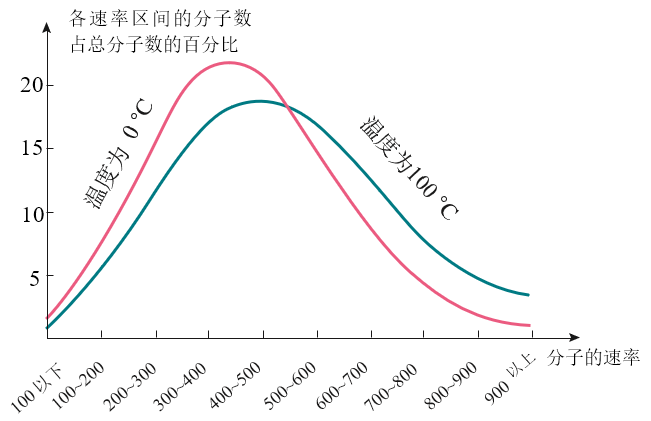
\includegraphics[width=\textwidth,keepaspectratio]{./pictures/23.png}
          \end{minipage}
          \hfill
          \begin{minipage}{0.45\textwidth}
              \begin{enumerate}[label = (\arabic*)]
                  \item 中间高,两头低
                  \item[]
                  \item 温度越高,峰值点下降并横移
                  \item[]
                  \item 任何温度下,图像围成的面积为$1$
              \end{enumerate}
          \end{minipage}
\end{itemize}

\vspace{2em}

\subsubsection{温度和温标}
\begin{enumerate}
    \item 气体的状态参量
          \begin{itemize}
              \item 几何性质: 体积
              \item 力学性质: 压强
              \item 热学性质: 温度
              \item $\dfrac{PV}{T} = C \,$ ($C$常数,与质量和气体种类相关)
          \end{itemize}
    \item 温度
          \begin{itemize}
              \item 意义: 宏观上表示物体的冷热程度,微观上表示的是分子热运动的剧烈程度
              \item 温标: 摄氏温度$t \, ^{\circ}$,热力学温标$T$,单位$K$(开)
              \item 转化: $T = t + 273.15 \,$(绝对零度: $T = 0 \lra t = -273.15^{\circ} $)
          \end{itemize}
    \item 热平衡: 两个热力学系统之间无温度差(温度相同)
\end{enumerate}

\vspace{2em}

\subsubsection{内能}
\begin{enumerate}
    \item 分子平均动能: 温度有关
    \item 分子势能: 由分子的\textbf{位置}决定,在微观上与\textbf{分子间距}相关,宏观上与\textbf{体积}相关
    \item 内能的概念: 物体\textbf{所有分子}的 热运动的\textbf{动能与分子势能}的总和
    \item 内能的决定因素:
          \begin{enumerate}[label = (\arabic*)]
              \item 微观上: 分子个数,分子平均动能,分子势能
              \item 宏观上: 质量,温度,体积
          \end{enumerate}
    \item 理想气体: 有质量,分子无体积,分子之间没有作用力的气体
    \item 两个意义: 分子无体积(仍有占有体积)意味着气体可以无限被压缩
    
          \hspace{4.7em}分子间无作用力(气体内能\textbf{不包含分子势能})
    \item 结论: 理想气体内能只有动能项,其内能大小仅和温度有关
\end{enumerate}

\vspace{2em}

\subsection{物态及物态的变化}
\subsubsection{晶体与非晶体}
\begin{enumerate}
    \item 固体
          \begin{itemize}
              \item 根据有无固定熔点分为: 晶体(有) \, 非晶体(无)
              \item 根据有无规则的外形分为: 单晶体(有) \, 多晶体(无)

                    \vspace{-1em}
                    \hspace{-0.9em}\begin{adjustbox}{minipage=0.76\linewidth, bgcolor=gray!20, padding=1em}
                        \small % 将字号变小为 small
                        单晶体: 其内部微粒有规律地排列在一个空间格子内的晶体.

                        \hspace{3.8em}其晶体结构是连续的,或者可以说,在宏观尺度范围内单晶不包含晶界.

                        \,

                        多晶体: 仅存在于固体,由多颗大小及方向各异的晶粒所构成

                        \hspace{3.8em}而这些晶粒一般都由大量微小的单晶或微晶(微结晶、结晶粒、结晶子)组成.

                        \hspace{3.8em}在材料不同位置生长的结晶粒相遇时形成晶界
                    \end{adjustbox}
                    \vspace{-1em}

              \item 常见晶体: 石英 \, 食盐 \, 明矾 \, 云母 \, 天然水晶
              \item 常见非晶体: 蜂蜡 \, 橡浆 \, 玻璃
              \item 互相转换:

                    \hspace{4.8em}糖块 \, 是多晶体;组成糖块的颗粒 \, 是单晶体

                    \hspace{4.8em}天然水晶 \, 是单晶体;融化后再凝固的玻璃 \, 是非晶体
          \end{itemize}

    \item 各向同性与各向异性:
          \begin{itemize}
              \item 定义: 各个方向上的物理性质的同异(主要指导电性,导热性,透光性等)
              \item 单晶体: 其具有规则外形,因此不同方向上物理性质具有差异,各向异性
              \item 多晶体与非晶体: 其具有不规则外形,因此不同方向上物理性质一致,各向同性
          \end{itemize}

    \item 总结:

          \hspace{3em}\begin{tabular}{|c|c|c|c|}
              \hline
                   & 单晶体  & 多晶体  & 非晶体  \\
              \hline
              外形   & 规则   & 无规则  & 无规则  \\
              \hline
              固定熔点 & 有    & 有    & 无    \\
              \hline
              物理性质 & 各向异性 & 各向同性 & 各向同性 \\
              \hline
          \end{tabular}
\end{enumerate}

\vspace{2em}

\subsubsection{液体}
\begin{enumerate}
    \item 表面张力
          \begin{enumerate}[label = (\arabic*)]
              \item 生活中的现象: 球形露珠,水面上的水蜘蛛
              \item 作用: 表面张力是的液体具有\textbf{收缩}的趋势
              \item 效果: 使得表面积趋于最小,而在体积$V$相同的情况下,\textbf{球体表面积最小}
              \item 成因: 表面层蒸发使得分子较为稀疏,间距较大,表现为分子间的引力
              \item 方向: 与液体表面相切,与液体的分界线垂直
              \item 大小: 温度越高张力越小(例如蒸发现象),有杂质的时候张力更小(类似隔断)
          \end{enumerate}
    \item 浸润与不浸润
          \begin{enumerate}[label = (\arabic*)]
              \item 浸润现象: 毛巾洗脸,下雨衣服湿了,试管凹液面
              \item 不浸润现象: 荷叶上的水滴,水银凸液面
              \item 成因: 固体分子对液体分子的作用力

                    \begin{center}
                        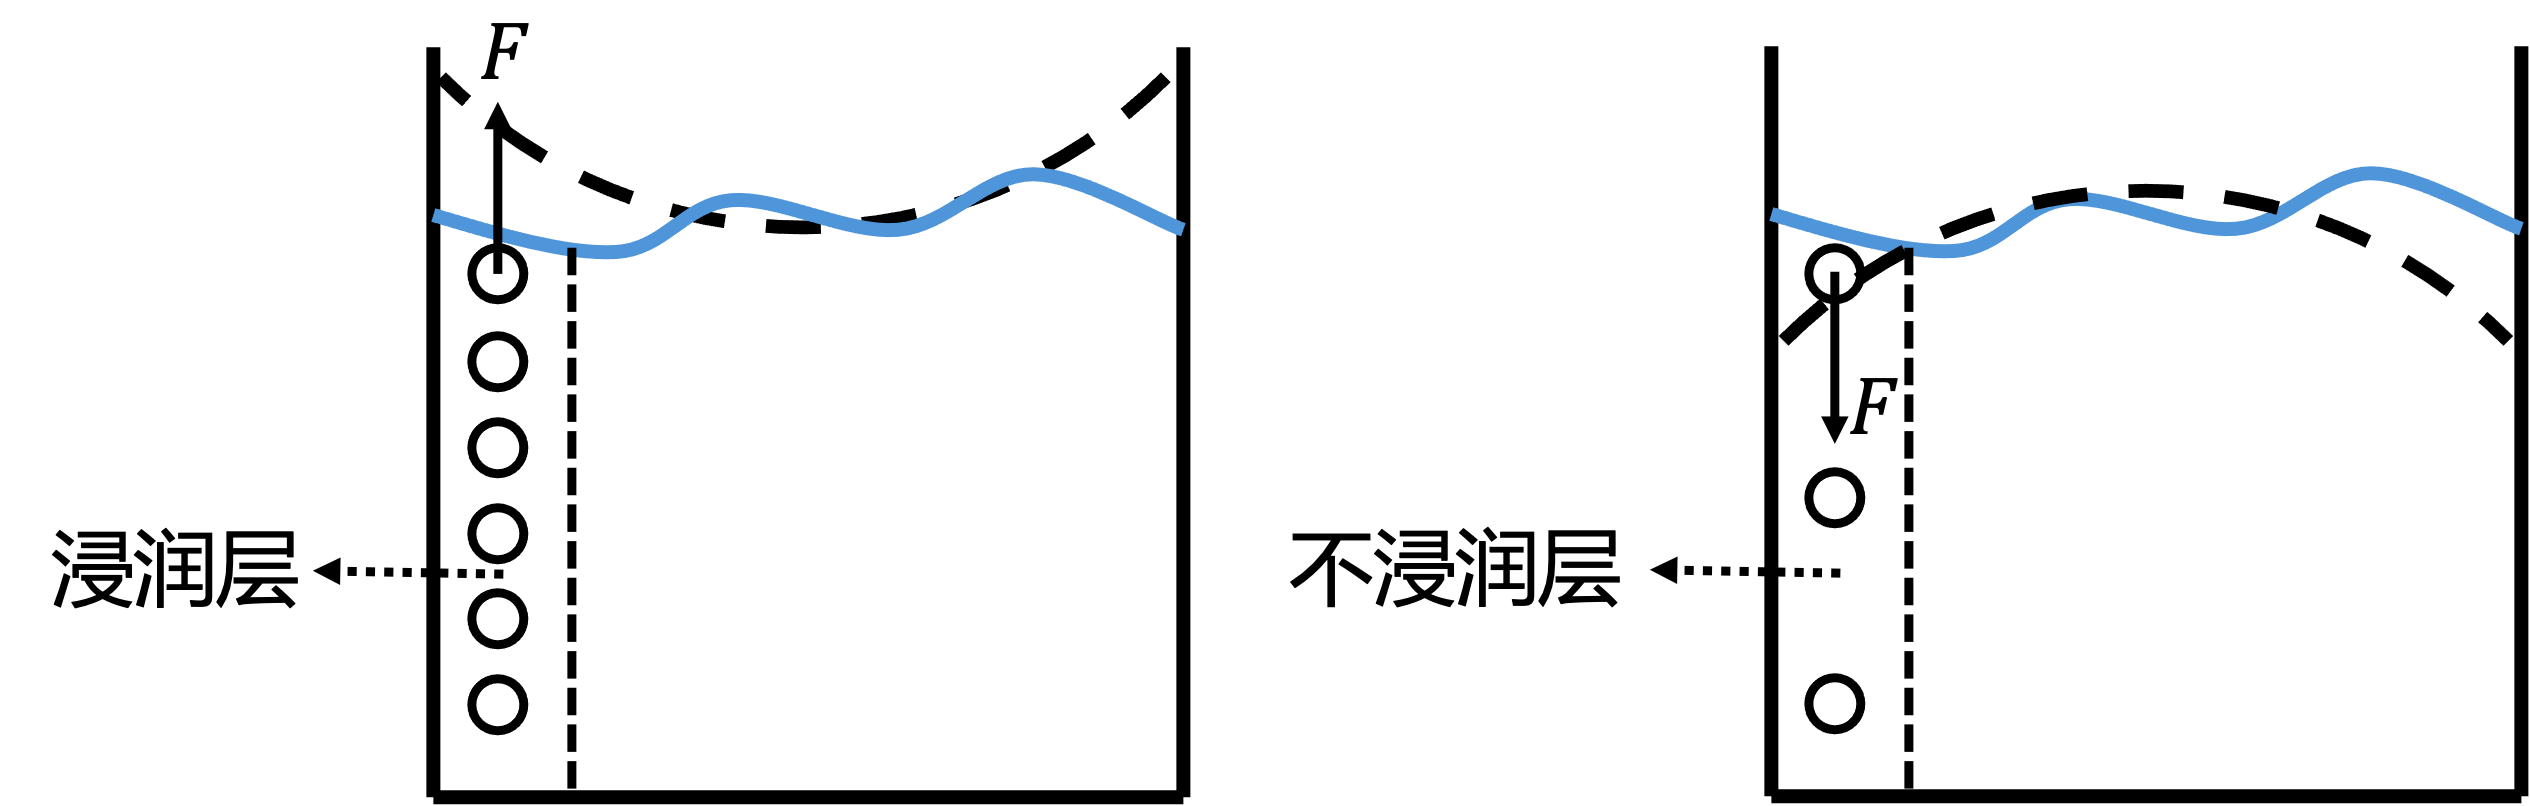
\includegraphics[width = 0.8\textwidth]{./pictures/24.png}
                    \end{center}

              \item 毛细现象: 本质上是 \, \textbf{浸润} \,和\, \textbf{表面张力} \, 的共同作用

                    \hspace{4.7em}\begin{minipage}{0.7\textwidth}
                        浸润时尽可能贴附固体分子(水液面上升)

                        非浸润时尽可能排斥固体分子(水银液面下降)

                        试管越细,那么管内的液体则越少,毛细现象越明显

                        \vspace{-1em}
                        \hspace{-0.9em}\begin{adjustbox}{minipage=0.7\linewidth, bgcolor=gray!20, padding=1em}
                            \small 
                            液面上升高度 $\, h= \dfrac{2\gamma \cos{\theta}}{\rho gr} \quad $($\theta$:液面切线与固体面所成锐角)

                            $\gamma$:表面张力系数;$\quad \theta$:接触角;$\quad \rho$:液体密度;$\quad r$:试管半径
                        \end{adjustbox}
                        \vspace{-1em}

                        下雨\textbf{踩土}(减少土壤缝隙宽度)\textbf{加强}毛细现象,减少树木根部积水

                        下雨\textbf{刨土}(使得土壤不再有缝隙)\textbf{破坏}毛细现象,增加树木根部水量
                    \end{minipage}
          \end{enumerate}

    \item 液晶: 像液体一样具有流动性,光学性质与单晶体相似具有各向异性

          \hspace{2.4em} 液晶不是单/多晶体与非晶体,独立种类

          \begin{center}
              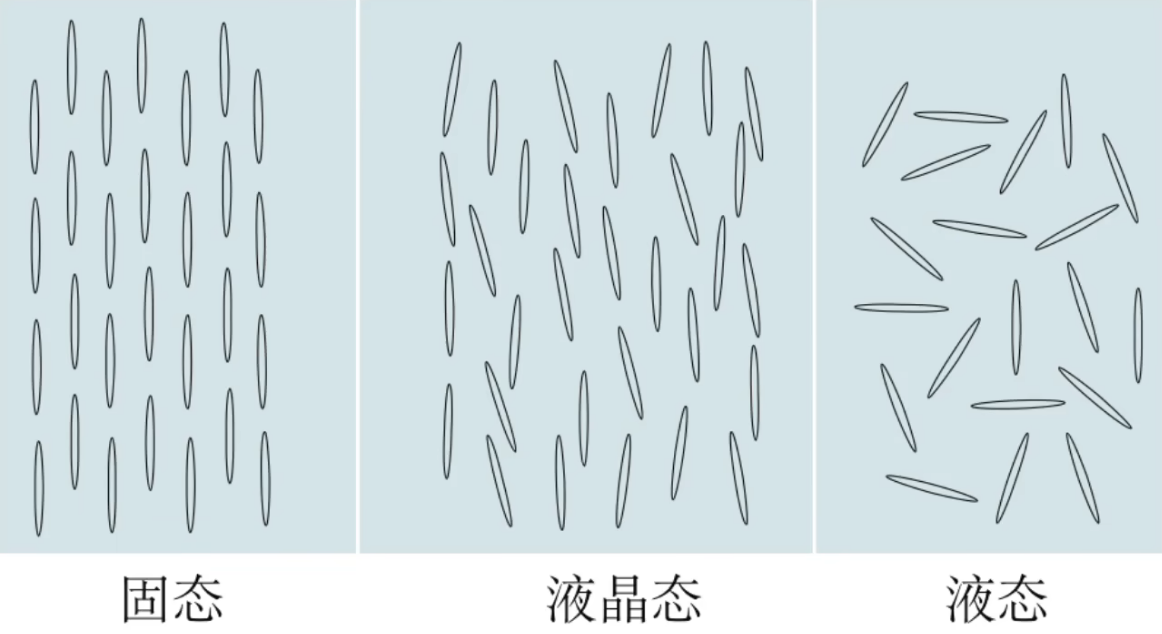
\includegraphics[width = 0.5\textwidth]{./pictures/25.png}
          \end{center}
\end{enumerate}

\vspace{2em}

\subsubsection{饱和汽与饱和汽压}
\begin{enumerate}
    \item 概念:
          \begin{enumerate}[label = (\arabic*)]
              \item 饱和汽: 与液体处于动态平衡的蒸汽
              \item 饱和汽压: 饱和汽的压强
          \end{enumerate}
    \item 理解: 在溶液中既有水分子蒸发出去,也有水分子液化回来
          \begin{itemize}
              \item 蒸发(与温度相关): 蒸发的水分子数$>$液化水分子数
              \item 液化(与温度相关,与蒸汽密度相关): 液化的水分子数$>$蒸发水分子数
              \item 平衡: 蒸发的水分子数$=$液化水分子数
          \end{itemize}
    \item 饱和汽压的影响因素:
          \begin{itemize}
              \item 温度: 温度越高,蒸发与冷凝强度均高,分子密度也越大,蒸汽的饱和汽压越大
              \item 体积: 与液面上方的体积\textbf{无关}(改变体积会改变当前状态,稳态不变)
              \item 密度: 无关。增大体积,上方蒸汽密度下降,液化能力下降,蒸发能力不变
              
              \hspace{2.7em}上方净累积分子,稳态后,密度不变
          \end{itemize}
\end{enumerate}

\vspace{2em}

\subsubsection{相对湿度与绝对湿度}
\begin{itemize}
    \item 绝对湿度: 此时水蒸气的\textbf{压强}
    \item 相对湿度: 绝对湿度除以水的饱和汽压
    \item 相对湿度公式: $ \text{相对湿度} = \frac{\text{绝对湿度}}{\text{饱和汽压}} $
    \item 人体感觉潮湿或干燥: 感受到的是相对湿度
    \item 干湿泡温度计: 两根温度计,一根温度计裹着湿棉布,另一根测量室温

          \hspace{6.6em} 湿棉布蒸发吸热,温度计示数低,两根温度计示数差

          \hspace{6.6em} 温度差越大,蒸发现象越明显,无温差则无蒸发现象

          \hspace{6.6em} 因此绝对湿度与饱和汽压相差较大,比值是相对湿度会越小
\end{itemize}

\vspace{2em}

\subsection{理想气体}
\subsubsection{气体压强的微观解释}
\begin{enumerate}
    \item 理解气体压强
          \begin{enumerate}[label = (\arabic*)]
              \item 气压: 气体分子对物质界面不断的撞击
              \item 推导:

                    \begin{proof}
                        \begin{align*}
                            F\triangle t & =  Nmv  \quad(\text{分子碰撞后停止})                                 \\
                            N            & = n \triangle V = n \cross (v \triangle t S) = nvS\triangle t \\
                            P            & = \frac{F}{S} = nmv^{2}
                        \end{align*}
                    \end{proof}

              \item 影响压强的因素: $n$单位体积分子数(体积$V$),$v$分子热运动速度(温度$T$)

                    \vspace{-1em}
                    \hspace{-0.9em}\begin{adjustbox}{minipage=0.53\linewidth, bgcolor=gray!20, padding=1em}
                        \small
                        $n = \frac{N}{S \triangle t}$,$\quad n$也可以被定义成单位面积,单位时间撞击次数.
                    \end{adjustbox}
                    \vspace{-1em}

          \end{enumerate}
\end{enumerate}

\vspace{2em}

\subsubsection{压强的表示以及画法}
\begin{enumerate}
    \item 压强的表示方法
          \begin{enumerate}[label = (\arabic*)]
              \item 公式: $P = \frac{F}{S} \quad $ 单位: 帕斯卡$Pa$
              \item 表示方法
                    \begin{enumerate}
                        \item 帕斯卡: $Pa$
                        \item 一个大气压: $1atm = 10^{5}Pa$
                        \item 汞柱高度: $cmHg \,  (1atm = 76cmHg)$
                        \item 任意液柱: $\rho gh$
                    \end{enumerate}
          \end{enumerate}
    \item 压强的的画法: 气体\textbf{垂直}指向碰撞面
    \item 压强的等式
          \begin{enumerate}[label = (\arabic*)]
              \item 液面封闭气体
                    \begin{itemize}
                        \item 研究对象: 液柱
                        \item 列式模版: 大气压两侧平衡(包括液压)
                        \item 注意: 等式两边的单位制应该一致,同时用帕斯卡$Pa$或者$cmHg$,$h$取竖直高度
                    \end{itemize}
              \item 连通器
                    \begin{itemize}
                        \item 原理: 等高液面的压强是相等的
                        \item 研究对象: 等高液面
                        \item 列式模版: 连通器两侧对于等高液面的压强相等
                        \item 注意: $h$为高度差,以及液体的压强方向
                    \end{itemize}
              \item 活塞(考虑质量)
                    \begin{itemize}
                        \item 研究对象: 活塞(受力分析)
                        \item 列式模版: 压强转化为力,力学平衡等式
                        \item 注意: 活塞有一侧为斜面时,斜面积需要重新计算,同时该力进行分解
                    \end{itemize}
          \end{enumerate}
\end{enumerate}

\vspace{2em}

\subsubsection{气体三大实验定律}
\begin{enumerate}[label = \arabic*]
    \item 气体的状态参量
          \begin{enumerate}[label = (\arabic*)]
              \item 参量: $P \, V \, T$
              \item 关系: $\frac{PV}{T} = C$
              \item 适用条件: 同一气体且质量(物质的量)不变(当漏气时$C$下降)
          \end{enumerate}
    \item 玻意耳定律(人名要记忆)---$T$不变
          \begin{itemize}
              \item 概念: 温度一定时,一定质量的气体,$P,V$成反比$\lra PV = C$
              \item 记忆方式: \textbf{耳}的右边有类似$T$的存在
          \end{itemize}
    \item 查理定律(人名要记)---$V$不变
          \begin{itemize}
              \item 概念: 体积一定时,一定质量的气体,$P,T$成正比$\lra \frac{P}{T} = C$
              \item 记忆方式: \textbf{查}中间有个倒着的$V$
          \end{itemize}
    \item 盖-吕萨克定律(人名要记)---$P$不变
          \begin{itemize}
              \item 概念: 压强一定时,一定质量的气体,$V,T$成正比$\lra \frac{V}{T} = C$
              \item 记忆方式: \textbf{萨}左下角有个类似$P$的存在
          \end{itemize}
\end{enumerate}

\vspace{2em}

\subsubsection{液柱的移动}

\begin{itemize}
    \item 瞬态变化量的计算

          $ \frac{P}{T} = \frac{\triangle P}{\triangle T} \quad or \quad \frac{V}{T} = \frac{\triangle V}{\triangle T}  \quad $(过原点的函数才能这样写)

          等式只用做计算$\triangle P \,or\, \triangle T \, or \, \triangle V$瞬间变化程度,以此来判断液面移动方向

          并不代表稳态后的$\triangle P \,or\, \triangle T \,or\, \triangle V$

          若在瞬态过程中,有同时有多个量导致液面的上升或下降

          可以直接考虑末态方程,从结果上判断某些量的确定增减性,在进行判断液面

    \item 充放气问题-物质的量的变化

          克拉伯龙方程: $PV = n R T \quad $($n$:物质的量;$R$:气体常数)

          涉及气体物质的量的变化,待被充气体$P\triangle V = \triangle n RT \quad $($n,V,m$具有等价性)

\end{itemize}

\vspace{2em}

\subsection{热力学三大定律}
\subsubsection{热力学第一定律和能量守恒}

\begin{enumerate}[label = \arabic*]
    \item 改变物体内能的两种方式
          \begin{enumerate}[label = (\arabic*)]
              \item 做功(摩擦生热等)
              \item 热传递(热辐射等)
          \end{enumerate}
    \item 热力学第一定律
          \begin{enumerate}[label = (\arabic*)]
              \item 内容: 一个热力学系统的内能增量等于外界向它传递的热量与外界对它所做的功的和
              \item 表达式: $ \triangle u = W + Q $

                    \begin{center}
                        \begin{tabular}{|c|c|c|c|}
                            \hline
                            \,  & $W$     & $Q$  & $\triangle u$ \\
                            \hline
                            $+$ & 外界对物体做功 & 吸收热量 & 内能增加          \\
                            \hline
                            $-$ & 物体对外界做功 & 放出热量 & 内能减少          \\
                            \hline
                        \end{tabular}
                    \end{center}

              \item 气体膨胀/压缩时: 物体对外界做功/外界对物体做功
              \item 判断内能变化不同研究对象分析方式不同:
                    \begin{enumerate}[label = (\alph*)]
                        \item 研究对象为 \textbf{固体或液体} \, 时:

                              \begin{minipage}{0.8\textwidth}
                                  晶体(固定熔点)熔化时温度不变,吸热使得内能增大

                                  \vspace{-1em}
                                  \hspace{-1em}\begin{adjustbox}{minipage=0.38\linewidth, bgcolor=gray!20, padding=1em}
                                      \small
                                      破坏了空间点阵结构,增大了分子势能
                                  \end{adjustbox}
                                  \vspace{-1em}

                                  同质量的$0^{\circ}C$水和$0^{\circ}C$冰,后者吸热变成水,因此前者内能更大
                              \end{minipage}
                        \item 研究对象为 \textbf{理想气体} \, 时

                              $m$一定时,理想气体无分子势能,其内能只和温度有关
                    \end{enumerate}
              \item 做功公式: $W = P \vdot \triangle V \, $(必须要求恒压过程)
          \end{enumerate}
    \item 解题中的特殊字眼
          \begin{enumerate}[label = (\arabic*)]
              \item 绝热: 没有热传递 $Q = 0$
              \item 真空: 不做功 $W = 0$
              \item 膨胀: 对外做功 $W < 0$
          \end{enumerate}

    \item 能量守恒定律: 能量既不可能凭空消失,也不能凭空产生

          \hspace{6.7em}它只能从一种形式转换为另一种形式,总量保持不变
\end{enumerate}

\vspace{2em}

\subsubsection{热力学第二定律和永动机}
\begin{enumerate}[label = \arabic*]
    \item 概念:

          \hspace{2.7em}克劳修斯表述: 热量不能\textbf{自发}的从高温到低温(方向性表述)

          \hspace{2.7em}开尔文表述: 不可能从单一热源吸收能量,使之完全变成\textbf{有用功},而不产生其他影响

          \hspace{8.4em}热机的效率不可能达到$100 \%$
          \item: 易错概念:

          \hspace{4.7em}热量不能自发地从内能低的传到内能高的物体($\times$)

          \hspace{4.7em}根据热力学第二定律,各种形式的能可以互相转换($\times$)

          \hspace{4.7em}自然界中自发进行的与热现象有关的宏观物理过程都具有方向性(\checkmark)

          \hspace{4.7em}一切与热现象有关的宏观自然过程都是不可逆的(\checkmark)

    \item 永动机

          \begin{enumerate}[label = (\arabic*)]
              \item 第一类永动机[内部能量互相转换](无法造出来): 违背能量守恒,会有其他能量损耗
              \item 第二类永动机[从外界吸收能量,即将耗散的能量再作为输入](无法造出):

                    \hspace{6.2em}违背热二的热传递方向性问题,耗散能量无法完全利用
          \end{enumerate}
\end{enumerate}

\subsubsection{热力学第三定律}
概念: 绝对零度无法达到($0 \, k \, or \, -273^{\circ}$)

\end{document}